%| This is a header file for Latex documents  
%| It contains a number of common packages, settings, and custom macros that I frequently use.
\documentclass[12pt,journal]{IEEEtran}

\usepackage[cmex10]{amsmath}        %| American Mathematical Society package for fancy maths  b
\interdisplaylinepenalty=2500              %| Restores IEEE line spacing after amsmath

%| IEEE Citation package
\usepackage{cite}
\usepackage[above]{placeins}
\usepackage{array}
%\usepackage{dblfloatfix}
\usepackage{color}
\usepackage{graphicx}
\usepackage{float}
\usepackage{url}                         %| Improved URL handling
\usepackage{etoolbox}
\usepackage[font=footnotesize]{subcaption}
\usepackage{listings}
%\usepackage{fixltx2e}               %| Better tables than for LaTeX 2e
\usepackage{minted}
\usepackage{stfloats}
\usepackage{multicol}
\usepackage{fancyhdr}

\pagestyle{fancy} 
\cfoot{\thepage}
\renewcommand{\headrulewidth}{0pt}
\renewcommand{\footrulewidth}{0pt}

%| Highlighting for source code listings
\definecolor{mygreen}{rgb}{0,0.6,0}
\definecolor{ltgray}{rgb}{0.98,0.98,0.98}
\definecolor{dkgray}{rgb}{0.5,0.5,0.5}
\definecolor{mymauve}{rgb}{0.58,0,0.82}
\lstset{
  xleftmargin = 4pt,
  backgroundcolor=\color{ltgray},  % choose the background color; you must add \usepackage{color} or \usepackage{xcolor}
  basicstyle=\tiny\ttfamily, % the size of the fonts that are used for the code
  breakatwhitespace=true,         % sets if automatic breaks should only happen at whitespace
  breaklines=true,                 % sets automatic line breaking
  captionpos=b,                    % sets the caption-position to bottom
  commentstyle=\color{mygreen},    % comment style
  deletekeywords={...},            % if you want to delete keywords from the given language
  escapeinside={\%*}{*)},          % if you want to add LaTeX within your code
  extendedchars=true,              % lets you use non-ASCII characters; for 8-bits encodings only, does not work with UTF-8
  frame=single,                    % adds a frame around the code
  keepspaces=true,                 % keeps spaces in text, useful for keeping indentation of code (possibly needs columns=flexible)
  keywordstyle=\color{blue},       % keyword style
  language=Verilog,          % the language of the code(I modified the .sty for systemverilog, found the code on google)
  morekeywords={*,...,.*,memc_t, uword, word_16, logic, always_comb, always_FF, status_t, status_e, control_e, class, endclass, simphase_e, rand, typedef, enum, import, package, endpackage, result_t, sel_t},            % if you want to add more keywords to the set
  numbers=left,                    % where to put the line-numbers; possible values are (none, left, right)
  numbersep=4pt,                   % how far the line-numbers are from the code
  numberstyle=\tiny\color{dkgray}, % the style that is used for the line-numbers
  rulecolor=\color{black},         % if not set, the frame-color may be changed on line-breaks within not-black text (e.g. comments (green here))
  showspaces=false,                % show spaces everywhere adding particular underscores; it overrides 'showstringspaces'
  showstringspaces=false,          % underline spaces within strings only
  showtabs=false,                  % show tabs within strings adding particular underscores
  stepnumber=4,                    % the step between two line-numbers. If it's 1, each line will be numbered
  stringstyle=\color{mymauve},     % string literal style
  tabsize=2,                       % sets default tabsize to 2 spaces
  title=\lstname                   % show the filename of files included with \lstinputlisting; also try caption instead of title
}

\lstset{keywordstyle=\color{purple}}
\lstset{keywordstyle={[2]\color{purple}} }
\lstset{keywordstyle={[3]\color{magenta}} }
\lstset{keywordstyle={[4]\color{teal} }}
\lstset{keywordstyle={[5]\color{violet!40}} }

% Alter some LaTeX defaults for better treatment of figures:
    % See p.105 of "TeX Unbound" for suggested values.
    % See pp. 199-200 of Lamport's "LaTeX" book for details.
    %   General parameters, for ALL pages:
    \renewcommand{\topfraction}{0.9}  % max fraction of floats at top
    \renewcommand{\bottomfraction}{0.8} % max fraction of floats at bottom
    %   Parameters for TEXT pages (not float pages):
    \setcounter{topnumber}{2}
    \setcounter{bottomnumber}{2}
    \setcounter{totalnumber}{2}     % 2 may work better
    \setcounter{dbltopnumber}{2}    % for 2-column pages
    \renewcommand{\dbltopfraction}{0.9} % fit big float above 2-col. text
    \renewcommand{\textfraction}{0.07}  % allow minimal text w. figs
    %   Parameters for FLOAT pages (not text pages):
    \renewcommand{\floatpagefraction}{0.9}  % require fuller float pages
    % N.B.: floatpagefraction MUST be less than topfraction !!
    \renewcommand{\dblfloatpagefraction}{0.9} % require fuller float pages


%| Enables PDF metadata, thumbnails, and navigation
\newcommand\MYhyperrefoptions{
  bookmarks=true,
  bookmarksnumbered=true,
  pdfpagemode={UseOutlines},
  plainpages=false,
  pdfpagelabels=true,
  colorlinks=true,
  linkcolor={black},
  citecolor={black},
  urlcolor={blue},
  pdftitle={Team 3: End of Project Documentation},
  pdfsubject={Senior Design},                        
  pdfauthor={Ben Smith, Devin Moore},
  pdfkeywords={Logic Design, FPGA, Verilog}}                       

%| Calls hyperref package with the options specified above
\usepackage[\MYhyperrefoptions,pdftex]{hyperref}

%| Font settings
\renewcommand{\sfdefault}{phv}
\renewcommand{\rmdefault}{ptm}
\renewcommand{\ttdefault}{pcr}

%| Restores IEEE table formatting after usage of subcaption package
\captionsetup[table]{format=plain,labelformat=simple,justification=centering, labelsep=newline, singlelinecheck=false, textfont={sc}}

%| Required Lab Demo custom function
%| \demo{Name}{Physical deliverable}{Documentation deliverable}{Process}
%| =================================================================================================
%| for boxed text and stuch
\usepackage{fancybox}
\newenvironment{fminipage}%
{\begin{Sbox}\begin{minipage}}%
{\end{minipage}\end{Sbox}\Ovalbox{\TheSbox}}

%| Actual bawx
\newcommand{\demo}[4] {
\vspace{15px}
\begin{centering}
  \begin{fminipage}{.47\textwidth}
    \vspace{3px}
    \centering{\bfseries \large Laboratory Demo: #1}\\*
    \vspace{10px}
    \begin{tabular}{p{1.4cm}  p{6.3cm}}
      %|==Requirements for lab demo==
      \raggedright Specification:                  &#2\\
      \\
      \raggedright  Deliverable:                   &#3\\
      \\
      \raggedright Process :                       &#4\\
    \end{tabular}
  \end{fminipage}
\end{centering}
}

%| Single figure
%| \small{Location}{Caption}{Label}
%| =================================================================================================
\newcommand{\smallfig}[3] {
  \begin{figure}[htb]
    \includegraphics[width=.48\textwidth]{#1}
    \caption{#2}
    \label{#3}
  \end{figure}
}

%| Single figure
%| \simpletable{c||c}{Caption}{Label}{content}
%| =================================================================================================
\newcommand{\simpletable}[4] {
  \begin{table}[H]
    \caption{#2}
    \label{#3}
    \centering
    \begin{tabular}{#1}
      #4
    \end{tabular}
  \end{table}
}

%| Big figure
%| \small{Location}{Caption}{Label}
%| =================================================================================================
\newcommand{\bigfig}[3]{
  \begin{figure*}[!tb]
    \includegraphics[width=\textwidth]{#1}
    \caption{#2}
    \label{#3}
  \end{figure*}
}

% \newcommand{\bigfig}[3]{
%   %\begin{multicols}{1}
%   \noindent%
%   \begin{minipage}{\textwidth}
%     \makebox[\textwidth]{%
%       \includegraphics[keepaspectratio=true,scale=1]{#1}}
%     \captionof{figure}{#2}% only if needed
%     \label{#3}
%   \end{minipage}
%   %\end{multicols}
% }

%| Single figure
%| \simpletable{Caption}{c||c}{content}
%| =================================================================================================
\newcommand{\weeklytable}[3] {
  \begin{table}[!t]
    \caption{#1}
    \centering
    \begin{tabular}{#2}
      {\bfseries  Topic}    &{\bfseries Hours}     \\
      \hline
      #3
      \hline
    \end{tabular}
  \end{table}
}
\usepackage{tabularx}
\usepackage{pdfpages}
\usepackage{lipsum}
\usepackage{pdfpages}

\renewcommand{\arraystretch}{1.3}

\newcommand{\COURSE}{CPE142: Computer Organization}
\newcommand{\TITLE}{Term Project: Phase Two}
\newcommand{\DUEDATE}{December Fourth 2014}
\newcommand{\ABSTRACT}{\textit{A pipelined CPU is designed to implement a subset of the MIPS instruction set...}}

\begin{document}
\begin{titlepage}
	\begin{center}
		\vspace{20 cm}
		
		\textsc{\Large \COURSE}\\[1.3cm]
		\textsc{\Large \DUEDATE}\\[0.5cm]

		\vspace{5 mm}
		
		% Title
		\rule{415pt}{2pt}\\
		{ \Huge \bfseries \TITLE \\[0.2cm] }
		\rule{415pt}{2pt}\\
		
		\vspace{10mm}
		
		%| Author names
		\begin{minipage}{0.4\textwidth}
		\begin{flushleft} \Large
		
		\emph{Authors:}\\
			Ben	  	\textsc{smith} 55\% \\
			Devin	\textsc{moore} 45 \%
		\end{flushleft}
		\end{minipage}
		\begin{minipage}{0.4\textwidth}
		\begin{flushright} \Large
		
		%| Faculty names
		\emph{Instructor:} \\
			Dr. Behnam 	\textsc{Arad}
		\end{flushright}
		\end{minipage}
	\end{center}
	
	%| gives the names a bit of breathing room
	\vspace{25mm}
	
	\begin{center}
	\begin{minipage}{470pt}
		%| Automatic abstract entry from main document
		\begin{flushleft} \Large
			%\begin{abstract}
			%	\normalsize \bfseries
			%	\ABSTRACT \\
			%\end{abstract}
			
		\end{flushleft}
		
		%| Automatic keyword entry from main document
		\begin{flushleft} \Large
			% \begin{keywords}
			% 	\normalsize
			% 	\KEYWORDS \\
			% \end{keywords}
		\end{flushleft}
	\end{minipage}
	\end{center}
	%| Fill the remainder of the page
	\vfill
		
	% Bottom of the page sac state logo
	\begin{center}
		
\includegraphics[width=0.2\textwidth]{./library/logo}~\\[1cm]
	\end{center}
\end{titlepage}
\pagenumbering{roman}
\onecolumn
\tableofcontents
% \twocolumn
\listoffigures
% \newpage
% \listoflistings
\listoftables
\twocolumn
% \newpage
\clearpage

\pagenumbering{arabic}
\setcounter{page}{1}

\refstepcounter{section}%
\addcontentsline{toc}{section}{\protect\numberline{\thesection}Status Report}%

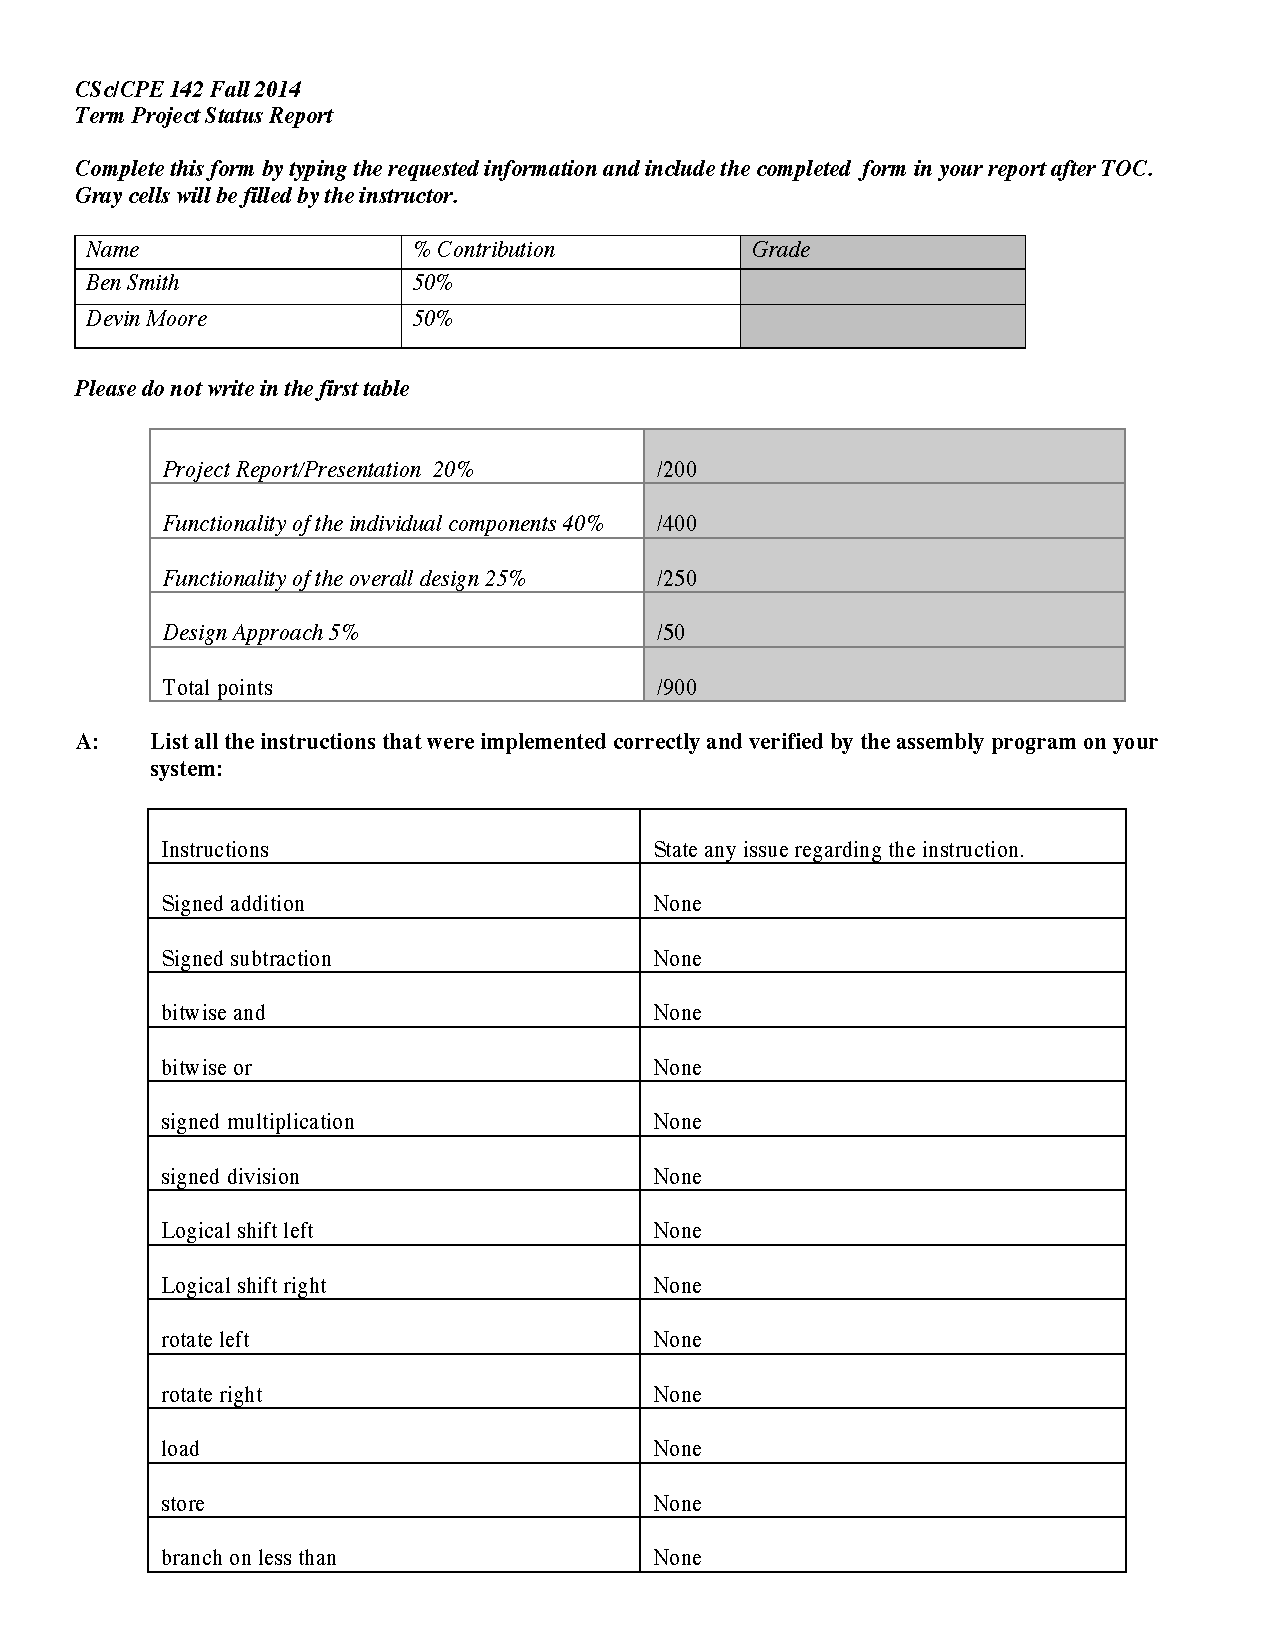
\includepdf[pages={1}]{figures/status_report.pdf}
\newpage
\includepdf[pages={2}]{figures/status_report.pdf}
\newpage

\section{Introduction}
\IEEEPARstart{T}{his} document details the design process of the CSUS CPE 142 Computer Organization 
course's term project. We have been asked to designed a pipelined datapath which implements an instruction 
set that is similar to MIPS in architecture. This project exercises a number of design principals from
the course material, particularly design considerations for hazard detection and mitigation. This
project started with several design specifications, the CPU had to be pipelined, hazards must be dealt
with and the supported instruction set was given. Other than the mentioned guidelines the students were
asked to make design decisions, the depth of the pipeline, which stage to put various components, and how
to mitigate potential hazards.

This document will first introduce the instruction set as specified in the project specification. This will 
present an opportunity to begin the discussion about the components that will be required to implement the
functionality described by the instructions. From this high level view of the architectue we will begin to
look at the functionality of the individual components of the system and what functionality they perform. 
After the individual blocks are described the processes of connecting them together and the dangers that
must be mitgated are discussed. 

\section{Instruction Set Architecture}
\IEEEPARstart{I}{nstruction} set architecture describes the fundamental elements of a processor's ability
to provide a service for software. This is also a sort of \textit{contract} between hardware and software
developers. As hardware developers we are saying this is what we promise to provide, our hardware can perform
these operations for you. As the instruction set is the focus of the hardware we are designing, it makes sense to
begin the design process with a through understanding of what hardware is to perform.

    \subsection{Supported Instruction Set Types}
    There are four instruction types in the prescribed instruction set, each of these types will support several 
    different operations. Most instructions will add to the hardware that must be implemented as they ask for more
    functionality. Our processor will start with the most basic components, program memory, program counter and the 
    hardware that's required to increment the program counter.

        \paragraph*{Instruction Format A}
        provides support for several arithmetic operations. All type A instructions carry an
        all zero opcode, the type of arithmetic operation is always decided by the four bit ``funct code'' field
        of the instruction. The organization of the instruction allows the func field to be supplied directly to
        the hardware which will perform the arithmetic without increasing the complexity of the main control logic.
        A full listing of supported hardware can be found in Table \ref{isa}.

        This instruction type introduces a need for the first two components of this processor, the Arithmetic and
        Logic Unit, or ALU, and a register file for providing input and recording the output of the ALU. 
        \begin{figure}[htpb]
            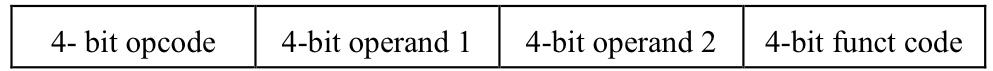
\includegraphics[width=.48\textwidth]{./figures/atype.jpg}
            \caption{A Type Instruction Format}
            \label{instructiontypes}
        \end{figure}

        \paragraph*{Instruction Format B}
        provides a way to load and store information from main memory. This greatly expands the capability of the
        ALU by removing the storage limitation of the register file. The new instructions require the implementation
        of some sort of addressable memory hardware to access. The two B type instructions, load word and
        store word, use indirect addressing schemes they will require the use of the ALU to calculate the physical
        address that is to be read or written to. The offset used in indirect addressing is signed and only
        4 bits it necessitates new hardware to handle the sign extension out to the 16 bit width required by the ALU.
        \begin{figure}[htpb]
            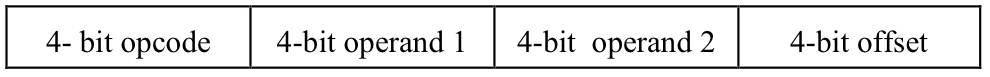
\includegraphics[width=.48\textwidth]{./figures/btype.jpg}
            \caption{B Type Instruction Format}
        \end{figure}

        \paragraph*{Instruction Format C}
        Allows the CPU to change the program counter based on logical outcomes. The instruction supplies an offset and
        a number to compare to a specific register, R0. The instructions jump when the instruction's operand 1 field is
        greater, equal, or less than R0 depending on the instruction. This comparison operation requires either the ALU
        or specialized hardware to provide these comparisons. There must also be additional hardware which will allow the 
        instruction to effect the program counter. The jump range of these instructions is increased by shifting the 8-bit
        offset field left on the natural word boundary of memory. This can be done because all instructions are the  same
        width.
        \begin{figure}[htpb]
            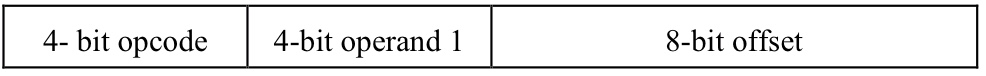
\includegraphics[width=.48\textwidth]{./figures/ctype.jpg}
            \caption{C Type Instruction Format}
        \end{figure}

        \paragraph*{Instruction Format D}
        allows the program counter to be set to almost anywhere in the program memory space. It does this by carrying a
        relatively large 13-bit effective jump offset. Although the opcode only allows for a 12-bit offset filed, the
        number is shifted to the left because instructions only start at even memory locations.

        \begin{figure}[htpb]
            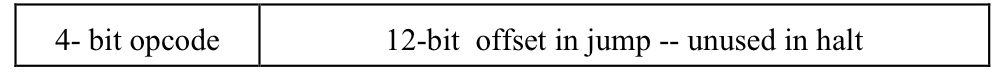
\includegraphics[width=.48\textwidth]{./figures/dtype.jpg}
            \caption{D Type Instruction Format}
        \end{figure}

    \begin{table*}[htbp]
        \caption{Full Set of Supported Instructions}
        \label{isa}
        \centering
        \begin{tabular}{r | l c c c c c p{5cm}}
            Function              & syntax             &opcode& op1   & op2    & f. Code & type   & Operation \\
            \hline
            Signed addition       & add op1, op2       & 0000 & reg  & reg    & 1111 & A & op1 = op1 $+$ op2 \\
            Signed subtraction    & sub op1, op2       & 0000 & reg  & reg    & 1110 & A & op1 = op1 - op2 \\
            bitwise and           & and op1, op2       & 0000 & reg  & reg    & 1101 & A & op1 = op1 \& op2 \\
            bitwise or            & or op1, op2        & 0000 & reg  & reg    & 1100 & A & op1 = op1 $|$ op2 \\
            signed multiplication & mul op1, op2       & 0000 & reg  & reg    & 0001 & A & op1 = op1 $*$ op2
 \\
                                  &                    &      &      &        &      &   & op1: Product (lower half) \\
                                  &                    &      &      &        &      &   & R0: Product (upper half) \\
            signed division       & div op1, op2       & 0000 & reg  & reg    & 0010 & A & op1: 16-bit quotient \\
                                  &                    &      &      &        &      &   & R0: 16-bit remainder \\
            Logical shift left    & sll op1, op2       & 0000 & reg  & immd   & 1010 & A & shift op1 to the left by op2 bits \\
            Logical shift right   & slr op1, op2       & 0000 & reg  & immd   & 1011 & A & shift op1 to the right by op2 bits with sign extension \\
            rotate left           & rol op1, op2       & 0000 & reg  & immd   & 1000 & A & rotate left op1 by op2 bits \\
            rotate right          & ror op1, op2       & 0000 & reg  & immd   & 1001 & A & rotate right op1 by op2 bits \\
            \hline
            load                  & lw op1, immd (op2) & 1000 & reg  & reg    & N/A  & B & op1 = Mem [ immd + op2] \\
                                  &                    &      &      &        &      &   & (sign extend immd) \\
            Store                 & sw op1, immd (op2) & 1011 & reg  & reg    & N/A  & B & Mem [immd + op2] = op1 \\
                                  &                    &      &      &        &      &   & (sign extend immd) \\
            \hline
            branch on less than   & blt op1, op2       & 0100 & reg  & immd.  & N/A  & C & if ( op1 $<$ R0 ) then \\
                                  &                    &      &      &        &      &   & PC = PC + op2\\
                                  &                    &      &      &        &      &   & (sign extend op2 \& shift left) \\
            branch on grater than & bgt op1, op2       & 0101 & reg  & immd.  & N/A  & C & if(op1 $>$ R0) then \\
                                  &                    &      &      &        &      &   & PC=PC+ op2 \\
                                  &                    &      &      &        &      &   & (sign extend op2 \& shift left) \\
            branch on equal       & beq op1, op2       & 0110 & reg  & immd.  & N/A  & C & if ( op1 = R0 ) then \\
                                  &                    &      &      &        &      &   & PC = PC + op2 \\
                                  &                    &      &      &        &      &   & (sign extend op2 \& shift left) \\
            \hline
            jump                  & jmp op1            & 1100 & off  & ------ & N/A  & D & pc = pc + op1 \\
                                  &                    &      &      &        &      &   & (S.E. op1 and left shift) \\
            halt                  & Halt               & 1111 & ---- & ------ & N/A  & D & halt program execution \\
            \hline
        \end{tabular}
    \end{table*}

\section{Memory and Register Design}
\IEEEPARstart{M}{emory} is so crucial to the operation of the system it was the first system block to undergo design. The project has a few requirements with regard to memory. These requirements dictate how the memory can be accessed and it's total capacity. The register file will require several custom logic functions to allow the ALU access to a special register for divide and multiplication operations that produce 32 bits of output. The following subsections detail the high level functionality of our processor's memory organization at an abstract level.

    \subsection{Main Memory}
    The system is based on a 16 bit architecture, the memory will make full use of the addressing lines and provide $2^{16}$ total bytes of memory. The memory is byte addressable but will always return a 16 bit word, the byte at the address port and the following byte.
    \begin{table}[H]
        \caption{Main Memory Module Ports}
        \label{mainmemory}
        \centering
        \begin{tabular}{r c p{4.5cm}}
        Signal      &Type    & Operation\\
        \hline
        write\_enable  & logic & write data into memory at the next positive edge clock \\
        write\_address & logic[16] & the address data will be written to if write is to take place \\
        write\_data    & logic[16] & the address data will be written to if write is to take place \\
        data\_out      & logic[16] & the 16 bit word at location write\_address will be made available\\
        \end{tabular}
    \end{table}

    \subsection{Program Memory}
    The program memory will be a combinatorial element which will output the instruction at a given address. There will be no synthasizable mechanism for loading this memory, it will be loaded by the system's testbench at simulation time.
    \begin{table}[H]
        \caption{Program Memory Module Ports}
        \label{programmemory}
        \centering
        \begin{tabular}{r c p{4.5cm}}
        Signal    &Type       & Operation\\
        \hline
        in & logic[16]& address from program counter, memory will return content at the specified location \\
        out & logic[16]& Instruction from address supplied at input port \\    
        \end{tabular}
    \end{table}

    \subsection{Register File}
    The register file's basic function is to provide the contents of a register when an address is supplied to it's address port. The register file has has two address ports and two data ports. Data will be produced on the output ports as soon as it is ready, not waiting for a clock. The write procedure is sequential and the data will be written on the rising edge of the system clock. The register will also implement two custom functions based around the R0 register. R0 will be accessible through the register ports like all of the other registers, but in addition to this it will respond to R0\_en and R0\_read.
    % \begin{figure}[H]
    %     \centering
    %     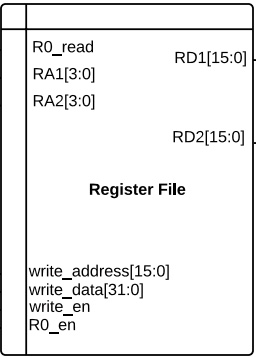
\includegraphics[width=.28\textwidth]{./figures/rf.jpg}
    %     \caption{Register File Block}
    %     \label{rffig}
    % \end{figure}

    \begin{table}[H]
        \caption{Register File Control Signals}
        \label{regfile}
        \centering
        \begin{tabular}{r c p{5cm}}
        Signal         & type      & Operation\\
        \hline
        RA1            & logic[4]  & read address for port 1\\
        RA2            & logic[4]  & read address for port 2\\
        RD1            & logic[16] & the 16 bit word at location write\_address will be made available\\
        RD2            & logic[16] & the 16 bit word at location write\_address will be made available\\
        write\_enable  & logic     & when asserted data from write\_data is captured on the falling edge of the clock \\
        write\_address & logic[4]  & the address data will be written to if write is to take place \\
        write\_data    & logic[16] & the data to be written at the positive edge of the clock \\
        \end{tabular}
    \end{table}

\section{Data Path Organization}
    \subsection{Number of Pipe Stages}
    The number of pipe stages the the primary design challenge of the first phase. A great deal of the difficulty surrounded assumptions that had to be made in the selection of the number of pipe stages. Pipelined designs are used to split combinational work across stages using flip flops to allow for higher global clock frequencies. We had to choose the number of pipe stages, guessing the longest path in the design. Given our understanding of digital logic we estimate that the ALU's signed divider circuit will require the most time by a wide margin. Because we do not intend to design a pipelined divider this operation is an atomic unit for us. 

    Because the ALU is assumed to require the longest time there is no logic between the inputs, outputs and the pipe flops ensuring highest possible operating frequency for the system. All of the control logic is implemented in the first stage and is assumed to require less time than the divisor circuit. 
    
    \subsection{Hazard detection and mitigation}    
    	The hazard detection unit is used to detect and handle any potential hazards that may occur due to pipelining. With the current three stage design, its outputs will be controlling register forwarding and stalling branch instructions for one cycle when a hazard is detected.
    	The most common hazard with this design is a data hazard. This occurs when an instruction is dependent on data from a previous instruction that has not yet been written back to the register file. When this occurs, the hazard detection unit will decide which control signals must be high in order to forward the correct data to where it will be used. These conditions can be found in Table \ref{HDU_COND}
    	
		\begin{table}[htpb]
		        \caption{Hazard Detection Unit Inputs}
		        \label{HDU_IN}
		        \centering
		        \begin{tabular}{r | p{6cm}}
		        Input          & Output is high when the following conditions are met\\
		        \hline
		        \hline
		        r0\_en			& This bit comes from the ALU control in the first stage. It is high for a MULTIPLY or DIVIDE instruction \\
		        \hline
		        instr[15:12] 	& This is the OPCODE from the first stage \\
		        \hline
		        S2.instr[15:12]	& This is the OPCODE from the second stage \\
		        \hline
		        S3.instr[15:12]	& This is the OPCODE from the third stage \\
		        \hline
		        instr[11:8]		& This is R1, typically the destination register address for instruction in first stage \\
		        \hline
		        instr[7:4]		& This is R2, typically the source register address for instruction in first stage \\
		        \hline
		        S2.instr[11:8]	& This is R1 of the second stage, typically the destination register \\
		        \hline		        		        		        
		        S3.instr[11:8] 	& This is R1 of the third stage, typically the destination register \\
		        \hline
		        \end{tabular}
		\end{table}
		    	
		\begin{table}[htpb]
		        \caption{Hazard Detection Unit Control Logic}
		        \label{HDU_COND}
		        \centering
		        \begin{tabular}{r | p{7cm}}
		        Signal          & Output is high when the following conditions are met\\
		        \hline
		        \hline
		        haz0			& Arithmetic or load followed two instructions later another arithmetic(Or STORE) using same destination register for R1. \\
		        \hline
		        haz1  			& Arithmetic or load directly followed by an arithmetic op with the R1 as the first destination. \\
		        \hline
		        haz2			& Arithmetic or load directly followed by an arithmetic op with the R2 as the first destination. \\
		        \hline
		        haz3			& Arithmetic or load followed 2 instructions later by an arithmetic op with the R2 as the first destination \\
		        \hline
		        haz4			& An Arithmetic operation is followed directly by a branch instruction   \\
		        \hline
		        haz5			& LOAD is followed directly, or second instruction, by a branch instruction using the dest register for compare. Also if an arithmetic op was followed 2 instructions later by a branch instruction using it's dest register \\
		        \hline
		        haz6			& Multiply or divide is followed directly by a branch instruction(What registers they specify does not matter. This is for R0 which is implicitly used by all 3 types) \\
		        \hline
		        haz7			& Multiply or divide is followed 2 instructions later by a branch instruction(What registers they specify does not matter. This is for R0 which is implicitly used by all 3 types) \\
		        \hline
		        haz8			& LOAD is followed directly by a STORE instruction using same reg for dest(load)/src(store) \\
		        \hline
		        haz9			& LOAD is followed 2 instructions later by a STORE instruction using same reg for 
		        dest(load)/src(store) \\
		        \hline
		        haz10			& Arithmetic instruction followed directly by a STORE instruction using same reg for dest/src \\
		        \hline
		        stall			& LOAD is followed directly by a branch instruction using the dest register for compare \\
		        \end{tabular}
		\end{table}
	\FloatBarrier
    \subsection{Stage 1}
    The first stage of this design contains nearly all of the control logic for processor. Since the path through
    the 16-bit signed divider of stage two is so long, a lot of control logic can be implemented without effecting
    the maximum frequency of the CPU. Much of this logic will be in parallel. The main control unit, the hazard detection unit, and most of the jump unit are all independent of each other and control separate signals. Most of the logic will be in the hazard detection unit, and will require inputs from all three stages before the outputs can drive anything. 
    
    
    \subsubsection{Main Control Unit and Exception Handling}
    The main control unit is responsible for decoding the opcode of the current instruction and controlling the data path. The truth table for this logic can be found in Table \ref{control}. The exception handling logic is omitted from this table due to size and complexity. Since the control unit is already handling the control signals for the halt operation, it also contains the logic to handle exceptions. There are three types of exceptions that are being handled; divide by zero, overflow, and unknown opcode.
    
    The ALU will be in charge of detecting a divide by zero, or an overflow. If the operation is to be a 16 bit signed division, it will check the divisor for a 0 and assert a div0 signal there is is an attempt to divide by zero. If an overflow is detected, it will assert the overflow flag. Both of these signals are sent to the main control unit, where it will halt the system by gating all of the clock inputs to the flops. It will do the same for the halt instruction, or any opcode that is unknown.
    
    \subsubsection{Sign Extender}
    The sign extender in the first stage must be able to handle 4, 8, and 16 bit inputs from the different types of instructions. The main control unit will provide the control signals to let the sign extender know which bits to extend. The logic can be seen in Table \ref{signextend}.
    
    
    \begin{figure*}[htpb]
        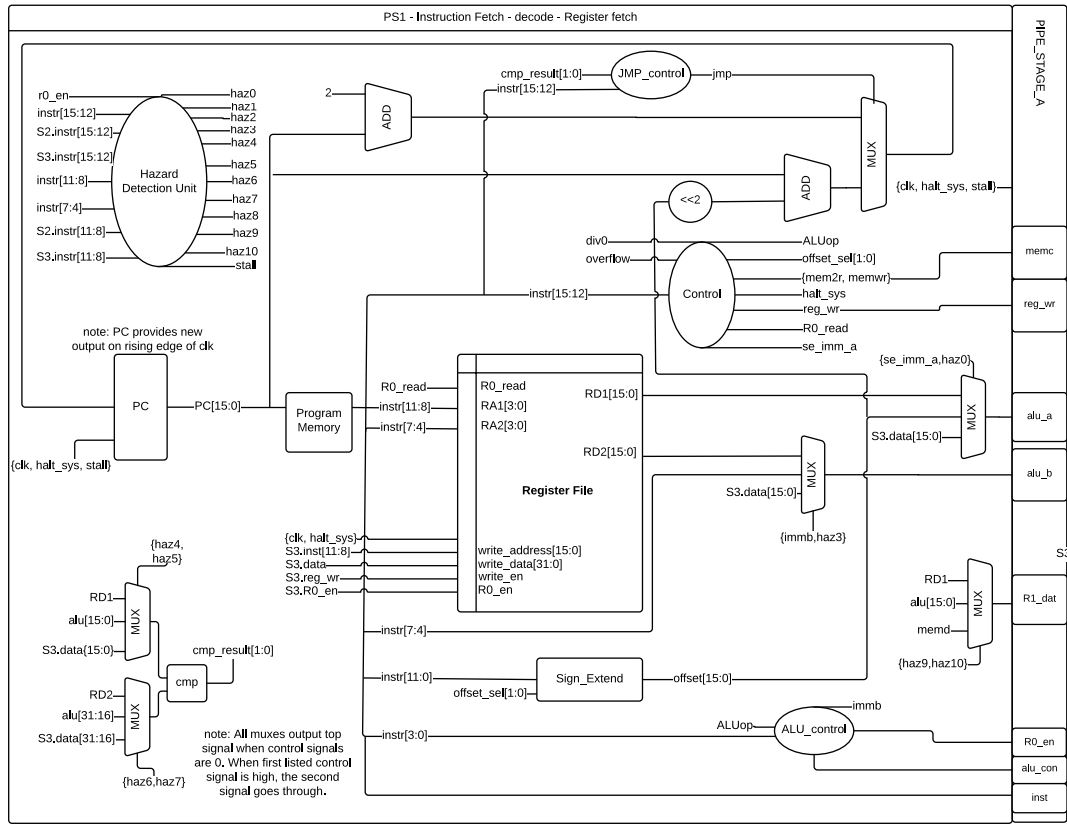
\includegraphics[width=\textwidth]{./figures/stage1.jpg}
        \caption{Pipeline Organization Stage One}
        \label{stage1}
    \end{figure*}

    \begin{table*}[htbp]
        \caption{Control Logic Truth Table}
        \label{control}
        \centering
        \begin{tabular}{r | c c c c | c c c c c c c}
                  & Input            &           &           &           & Output &                 &       &       &         &        & \\
            Instruction & instr[15] & instr[15] & instr[15] & instr[15] & ALUop  & offset\_sel[1:0] & mem2r & memwr & R0\_read & reg\_wr & se\_imm\_a \\
            \hline
            Type A      & 0                & 0         & 0         & 0         & 0      & 00              & 0     & 0     & 0       & 1      & 1 \\
            Load        & 1                & 0         & 0         & 0         & 1      & 10              & 1     & 0     & 0       & 1      & 0 \\
            store       & 1                & 0         & 1         & 1         & 1      & 10              & 0     & 1     & 0       & 0      & 0 \\
            BLT         & 0                & 1         & 0         & 0         & 0      & 10              & 0     & 0     & 1       & 0      & 1 \\
            BGT         & 0                & 1         & 0         & 1         & 0      & 10              & 0     & 0     & 1       & 0      & 1 \\
            BE          & 0                & 1         & 1         & 0         & 0      & 10              & 0     & 0     & 1       & 0      & 1 \\
            JMP         & 1                & 1         & 0         & 0         & 0      & 11              & 0     & 0     & 0       & 0      & 1 \\
            Halt        & 1                & 1         & 1         & 1         & 0      & 00              & 0     & 0     & 0       & 0      & 1 \\
        \end{tabular}
    \end{table*}


	\subsubsection{ALU Control Unit}
	The ALU control unit directly controls the operations of the ALU. It receives an ALUop bit from the main control unit to signal the use of the instruction's function code. If this bit is low, the ALU control signals will be determined by the function code, if it is high, the operation will be addition for the case of store and load instructions.
	For branching instructions, these signals don't matter because the main ALU results are not used. It would be more energy efficient to use another bit for those operations to completely shut off the ALU, but there are no energy constraints on our design. 
	
	There are 5 output signals from the ALU control unit, four of which 
	are input signals to the main ALU that determine its operations. The fifth output bit, imm\_b, is used to bring the immediate value from the instruction into the ALU for the shift and rotate functions. Since there are separate function for rotating left and right, there is no need to treat the immediate as a signed number and it is not sign extended.
	
    \begin{table*}[htbp]
        \caption{ALU Control Logic Truth Table}
        \label{alucontrol}
        \centering
        \begin{tabular}{r | c c c c c | c c c c c}
        Input & & & & & & Output & & & & \\
        \hline
        Instruction & ALUop & instr[3] & instr[2] & instr[1] & instr[0] & alu\_ctrl[3] & alu\_ctrl[2] & alu\_ctrl[1] & alu\_ctrl[0] & imm\_b\\
        SW/LW       & 1     & X        & X        & X        & X        & 0            & 0            & 0            & 0            & 0\\
        Add         & 0     & 1        & 1        & 1        & 1        & 0            & 0            & 0            & 0            & 0\\
        sub         & 0     & 1        & 1        & 1        & 0        & 0            & 0            & 0            & 1            & 0\\
        AND         & 0     & 1        & 1        & 0        & 1        & 0            & 0            & 1            & 0            & 0\\
        OR          & 0     & 1        & 1        & 0        & 0        & 0            & 0            & 1            & 1            & 0\\
        MULT        & 0     & 0        & 0        & 0        & 1        & 0            & 1            & 0            & 0            & 0\\
        DIV         & 0     & 0        & 0        & 1        & 0        & 0            & 1            & 0            & 1            & 0\\
        SHL         & 0     & 1        & 0        & 1        & 0        & 0            & 1            & 1            & 0            & 1\\
        SHR         & 0     & 1        & 0        & 1        & 1        & 0            & 1            & 1            & 1            & 1\\
        ROL         & 0     & 1        & 0        & 0        & 0        & 1            & 0            & 0            & 0            & 1\\
        ROR         & 0     & 1        & 0        & 0        & 1        & 1            & 0            & 0            & 1            & 1\\
        \end{tabular}
    \end{table*}


    
    \begin{table*}[htbp]
        \caption{Jump Control Logic}
        \label{jmp}
        \centering
        \begin{tabular}{r | c c c c c c | c }
                    & Input     &           &           &           &                &                & Output\\
                    \hline
        Instruction & instr[15] & instr[14] & instr[13] & instr[12] & cmp\_result[1] & cmp\_result[0] & jmp\\
        BLT         & 0         & 1         & 0         & 0         & 0              & 0              & 0\\
        BLT         & 0         & 1         & 0         & 0         & 0              & 1              & 1\\
        BLT         & 0         & 1         & 0         & 0         & 1              & 0              & 0\\
        BLT         & 0         & 1         & 0         & 0         & 1              & 1              & 0\\
        BGT         & 0         & 1         & 0         & 1         & 0              & 0              & 1\\
        BGT         & 0         & 1         & 0         & 1         & 0              & 1              & 0\\
        BGT         & 0         & 1         & 0         & 1         & 1              & 0              & 0\\
        BGT         & 0         & 1         & 0         & 1         & 1              & 1              & 0\\
        BE          & 0         & 1         & 1         & 0         & 0              & 0              & 0\\
        BE          & 0         & 1         & 1         & 0         & 0              & 1              & 0\\
        BE          & 0         & 1         & 1         & 0         & 1              & 0              & 1\\
        BE          & 0         & 1         & 1         & 0         & 1              & 1              & 0\\
        JMP         & 1         & 1         & 0         & 0         & 0              & 0              & 1\\
        JMP         & 1         & 1         & 0         & 0         & 0              & 1              & 1\\
        JMP         & 1         & 1         & 0         & 0         & 1              & 0              & 1\\
        JMP         & 1         & 1         & 0         & 0         & 1              & 1              & 1\\
        \end{tabular}
    \end{table*}
	
	\subsubsection{Branching and Jump Control Unit}
    The jump control unit decides whether to take PC + 2 or PC + offset during a branch or jump instruction. 
    This unit will be part of the critical path for this particular stage. Using the opcode input, it will determine what instruction is being performed and how to drive the jmp output based off the result from the comparator if necessary. The comparator results will be valid after the register file has been indexed, any hazards have been dealt with, and the register contents have propagated through the comparator. The truth table can be seen in Table \ref{jmp}. 
    
    All of the branching and jumping logic is handled within this first stage thanks to the large division path of the second stage. The comparator will output either a 00 for equal, 
    01 for R1 > R0, and a 10 for R1 < R0. The jump control unit will compare those results to the opcode to determine whether or not a branch will be taken. If the opcode is for JMP, it will assert the jmp control bit no matter what the comparator says.
    
    \begin{table}[htbp]
        \caption{Sign Extention Logic Table}
        \label{signextend}
        \centering
        \begin{tabular}{c c | c }
        Input         &               & Output\\
        \hline
        offset\_sel[1] & offset\_sel[0] & Action\\
        0             & 0             & nothing\\
        0             & 1             & extend 4 bits to 16\\
        1             & 0             & extend 8 bits to 16\\
        1             & 1             & extend 12 bits to 16\\
        \end{tabular}
    \end{table}
        
	% \begin{figure}[htpb]
 %        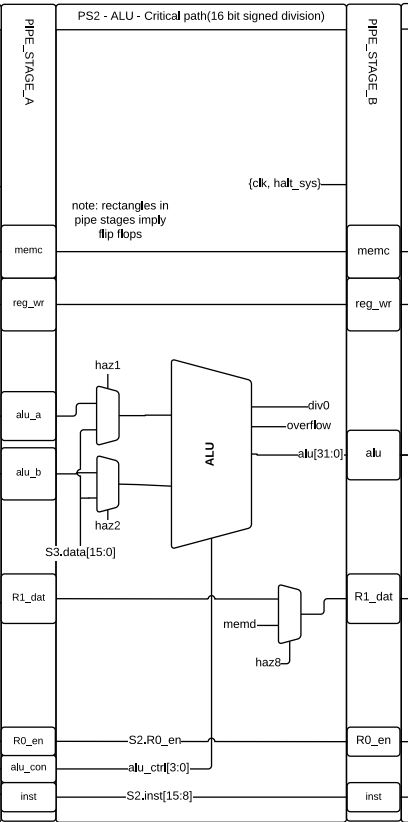
\includegraphics[width=.4\textwidth]{./figures/stage2.jpg}
 %        \caption{Pipeline Organization Stage Two}
 %        \label{stage2}
 %    \end{figure}
    
    \subsection{Stage 2}
    The entire second stage of this design belongs to the Arithmetic Logic Unit as seen in Figure
    \ref{stage2}. This ALU supports all of the operations listed in Table \ref{alucontrol}. Its function is 
    determined by the ALU\_control in the first stage. The 16 bit signed division will be our longest combinatorial path between stages, so there is very little logic between the ALU and the flip-flops.  
    
	% \begin{figure}[htpb]
 %        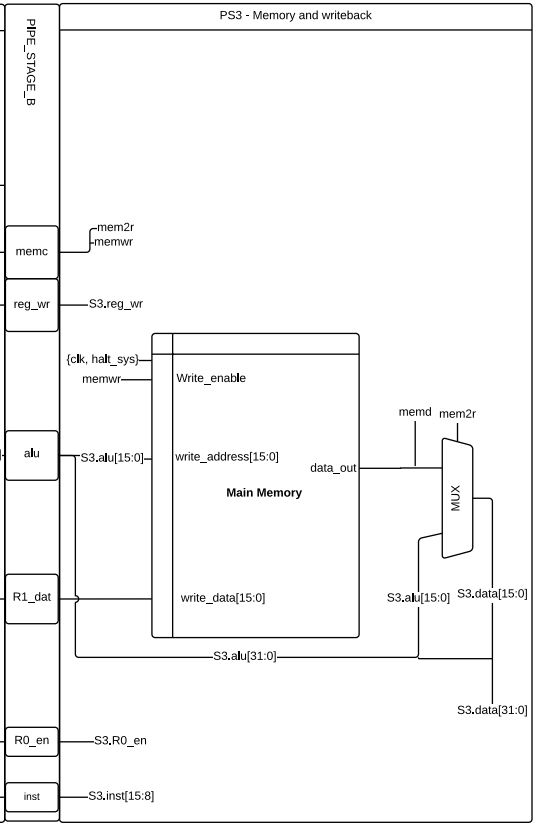
\includegraphics[width=.4\textwidth]{./figures/stage3.jpg}
 %        \caption{Pipeline Organization Stage Three}
 %        \label{stage3}
 %    \end{figure}    
	
    \subsection{Stage 3}
    The third stage of this pipelined processor handles memory references and writes back to the
    register file as seen in stage 3. The main logic of this stage is contained in the 
    main memory unit which is described in section two of this document.

	\section{Simulation and Verification}
        \subsection{Expected Results}
        We were given a small amount of assembly code to test our processor. We also
        received the initial values for the register file and main memory. 
        \lstinputlisting{../Paper/listings/program.asm}

        \begin{table}[htbp]
           \caption{Register File Contents}
           \label{regfi}
           \centering
           \begin{tabular}{ c | c }
           Register         & Expected \\
           \hline
           R1  &   0F00        \\
           R2  &   0050        \\
           R3  &   FF0F        \\
           R4  &   F0FF        \\
           R5  &   0040        \\
           R6  &   0024        \\
           R7  &   00FF        \\
           R8  &   AAAA        \\
           R9  &   0000        \\
           R10 &   0000        \\
           R11 &   0000        \\
           R12 &   FFFF        \\
           R13 &   0002        \\
           \end{tabular}
        \end{table}

        \begin{table}[htbp]
           \caption{Main Memory Contents}
           \label{mainme}
           \centering
           \begin{tabular}{ c | c }
           Address         & Contents   \\
           \hline
           00  &   2BCD                 \\
           All Others  &   0000         \\
           
           \end{tabular}
        \end{table}

        From the assembly code, we were able to translate it to binary program data 
        to be loaded into program memory. We used the following file to load the program memory.
        \lstinputlisting{../source/Verif/program_memory.hex}

        After determining what the given program code would do by hand, we had a good idea of
        what to look for. We were able to verify the end contents of the memory module and register file as seen in Table \ref{results}.

        %\lstinputlisting{../Paper/listings/program_breakdown.txt}

        \begin{table}[htbp]
        	   \caption{Final Register File Contents}
        	   \label{results}
        	   \centering
        	   \begin{tabular}{ c | c | c}
        	   Register         & Expected & Simulated   \\
        	   \hline
        	   R1  &   0001     &   0001        \\
               R2  &   0050     &   0050        \\
               R3  &   0050     &   0050        \\
               R4  &   21FE     &   21FE        \\
               R5  &   0900     &   0900        \\
               R6  &   0012     &   0012        \\
               R7  &   00FF     &   00FF        \\
               R8  &   597A     &   597A        \\
               R9  &   0000     &   0000        \\
               R10 &   597A     &   597A        \\
               R11 &   0051     &   0051        \\
               R12 &   FFFE     &   FFFE        \\
               R13 &   0002     &   0002        \\
        	   \end{tabular}
        	\end{table}
            \begin{table}[htbp]
               \caption{Final Main Memory Contents}
               \label{fmainme}
               \centering
               \begin{tabular}{ c | c | c }
               Address         & Expected & Results    \\
               \hline
               00  &   2BCD            \\
               02  &   597A            \\
               All Others  &   0000    \\
               
               \end{tabular}
            \end{table}
            The assignment prompt said to display every important signal at the falling
            edge of the clock for the entire program. The test bench will output these values
            during simulation. This is far too much data to print on paper.
             
            The give assembly program program will branch on the 16th instruction BGT which will skip 2 instructions. The program should halt on the 24th instruction because it is an unknown
            opcode which means the last two instructions will not finish.
            With this information we determined only 21 full instructions will run from start to finish. With 3 stages that should take 23 cycles.
            Our test bench system\_tb shows the halt to occur on the 23rd cycle. 


            \textbf{The main testbench in system\_tb.sv contains many singular tests up until 282ps. This is where the main assembly program starts running. }

	\section{Simulation and Verification}
	\subsection{Expected Results}
	We were given a small amount of assembly code to test our processor. We also
	received the initial values for the register file and main memory. 
	\lstinputlisting{../Paper/listings/program.asm}
	
	\begin{table}[htbp]
	   \caption{Register File Contents}
	   \label{regfi}
	   \centering
	   \begin{tabular}{ c | c }
	   Register         & Contents    \\
	   \hline
	   R1  &   0F00        \\
       R2  &   0050        \\
       R3  &   FF0F        \\
       R4  &   F0FF        \\
       R5  &   0040        \\
       R6  &   0024        \\
       R7  &   00FF        \\
       R8  &   AAAA        \\
       R9  &   0000        \\
       R10 &   0000        \\
       R11 &   0000        \\
       R12 &   FFFF        \\
       R13 &   0002        \\
	   \end{tabular}
	\end{table}
    \begin{table}[htbp]
       \caption{Main Memory Contents}
       \label{mainme}
       \centering
       \begin{tabular}{ c | c }
       Address         & Contents    \\
       \hline
       00  &   2BCD        \\
       All Others  &   0000        \\
       
       \end{tabular}
    \end{table}
    
    From the assembly code, we were able to translate it to binary program data to be loaded into program memory. We used the following file to load the program memory.
    \lstinputlisting{../source/Verif/program_memory.hex}
    
    After determining what the given program code would do by hand, we had a good idea of what to look for. We were able to verify the end contents of the memory module and register file as seen in Table \ref{results}.
    
    % \lstinputlisting{../Paper/listings/program_breakdown.txt}
    
	\begin{table}[htbp]
		   \caption{Final Register File Contents}
		   \label{results}
		   \centering
		   \begin{tabular}{ c | c | c}
		   Register         & Expected & Simulated   \\
		   \hline
		   R1  &   0001     &   0001        \\
	       R2  &   0050     &   0050        \\
	       R3  &   0050     &   0050        \\
	       R4  &   21FE     &   21FE        \\
	       R5  &   0900     &   0900        \\
	       R6  &   0012     &   0012        \\
	       R7  &   00FF     &   00FF        \\
	       R8  &   597A     &   597A        \\
	       R9  &   0000     &   0000        \\
	       R10 &   597A     &   597A        \\
	       R11 &   0051     &   0051        \\
	       R12 &   FFFE     &   FFFE        \\
	       R13 &   0002     &   0002        \\
		   \end{tabular}
		\end{table}
	    \begin{table}[htbp]
	       \caption{Final Main Memory Contents}
	       \label{fmainme}
	       \centering
	       \begin{tabular}{ c | c | c }
	       Address         & Expected & Results    \\
	       \hline
	       00  &   2BCD            \\
           02  &   597A            \\
	       All Others  &   0000    \\
	       \end{tabular}
	    \end{table}

	    The assignment prompt said to display every important signal at the falling
	    edge of the clock for the entire program. The test bench will output these values
	    during simulation. This is far too much data to print on paper.
	     
	    The give assembly program program will branch on the 16th instruction BGT which will skip 2 instructions. The program should halt on the 24th instruction because it is an unknown
	    opcode which means the last two instructions will not finish.
	    With this information we determined only 21 full instructions will run from start to finish. With 3 stages that should take 23 cycles.
	    Our test bench system\_tb shows the halt to occur on the 23rd cycle. 

        \textbf{The main testbench in system\_tb.sv contains many singular tests up until 282ps. This is where the main assembly program starts running. }

    \newpage  
    \begin{figure*}[htpb]
        \centering
        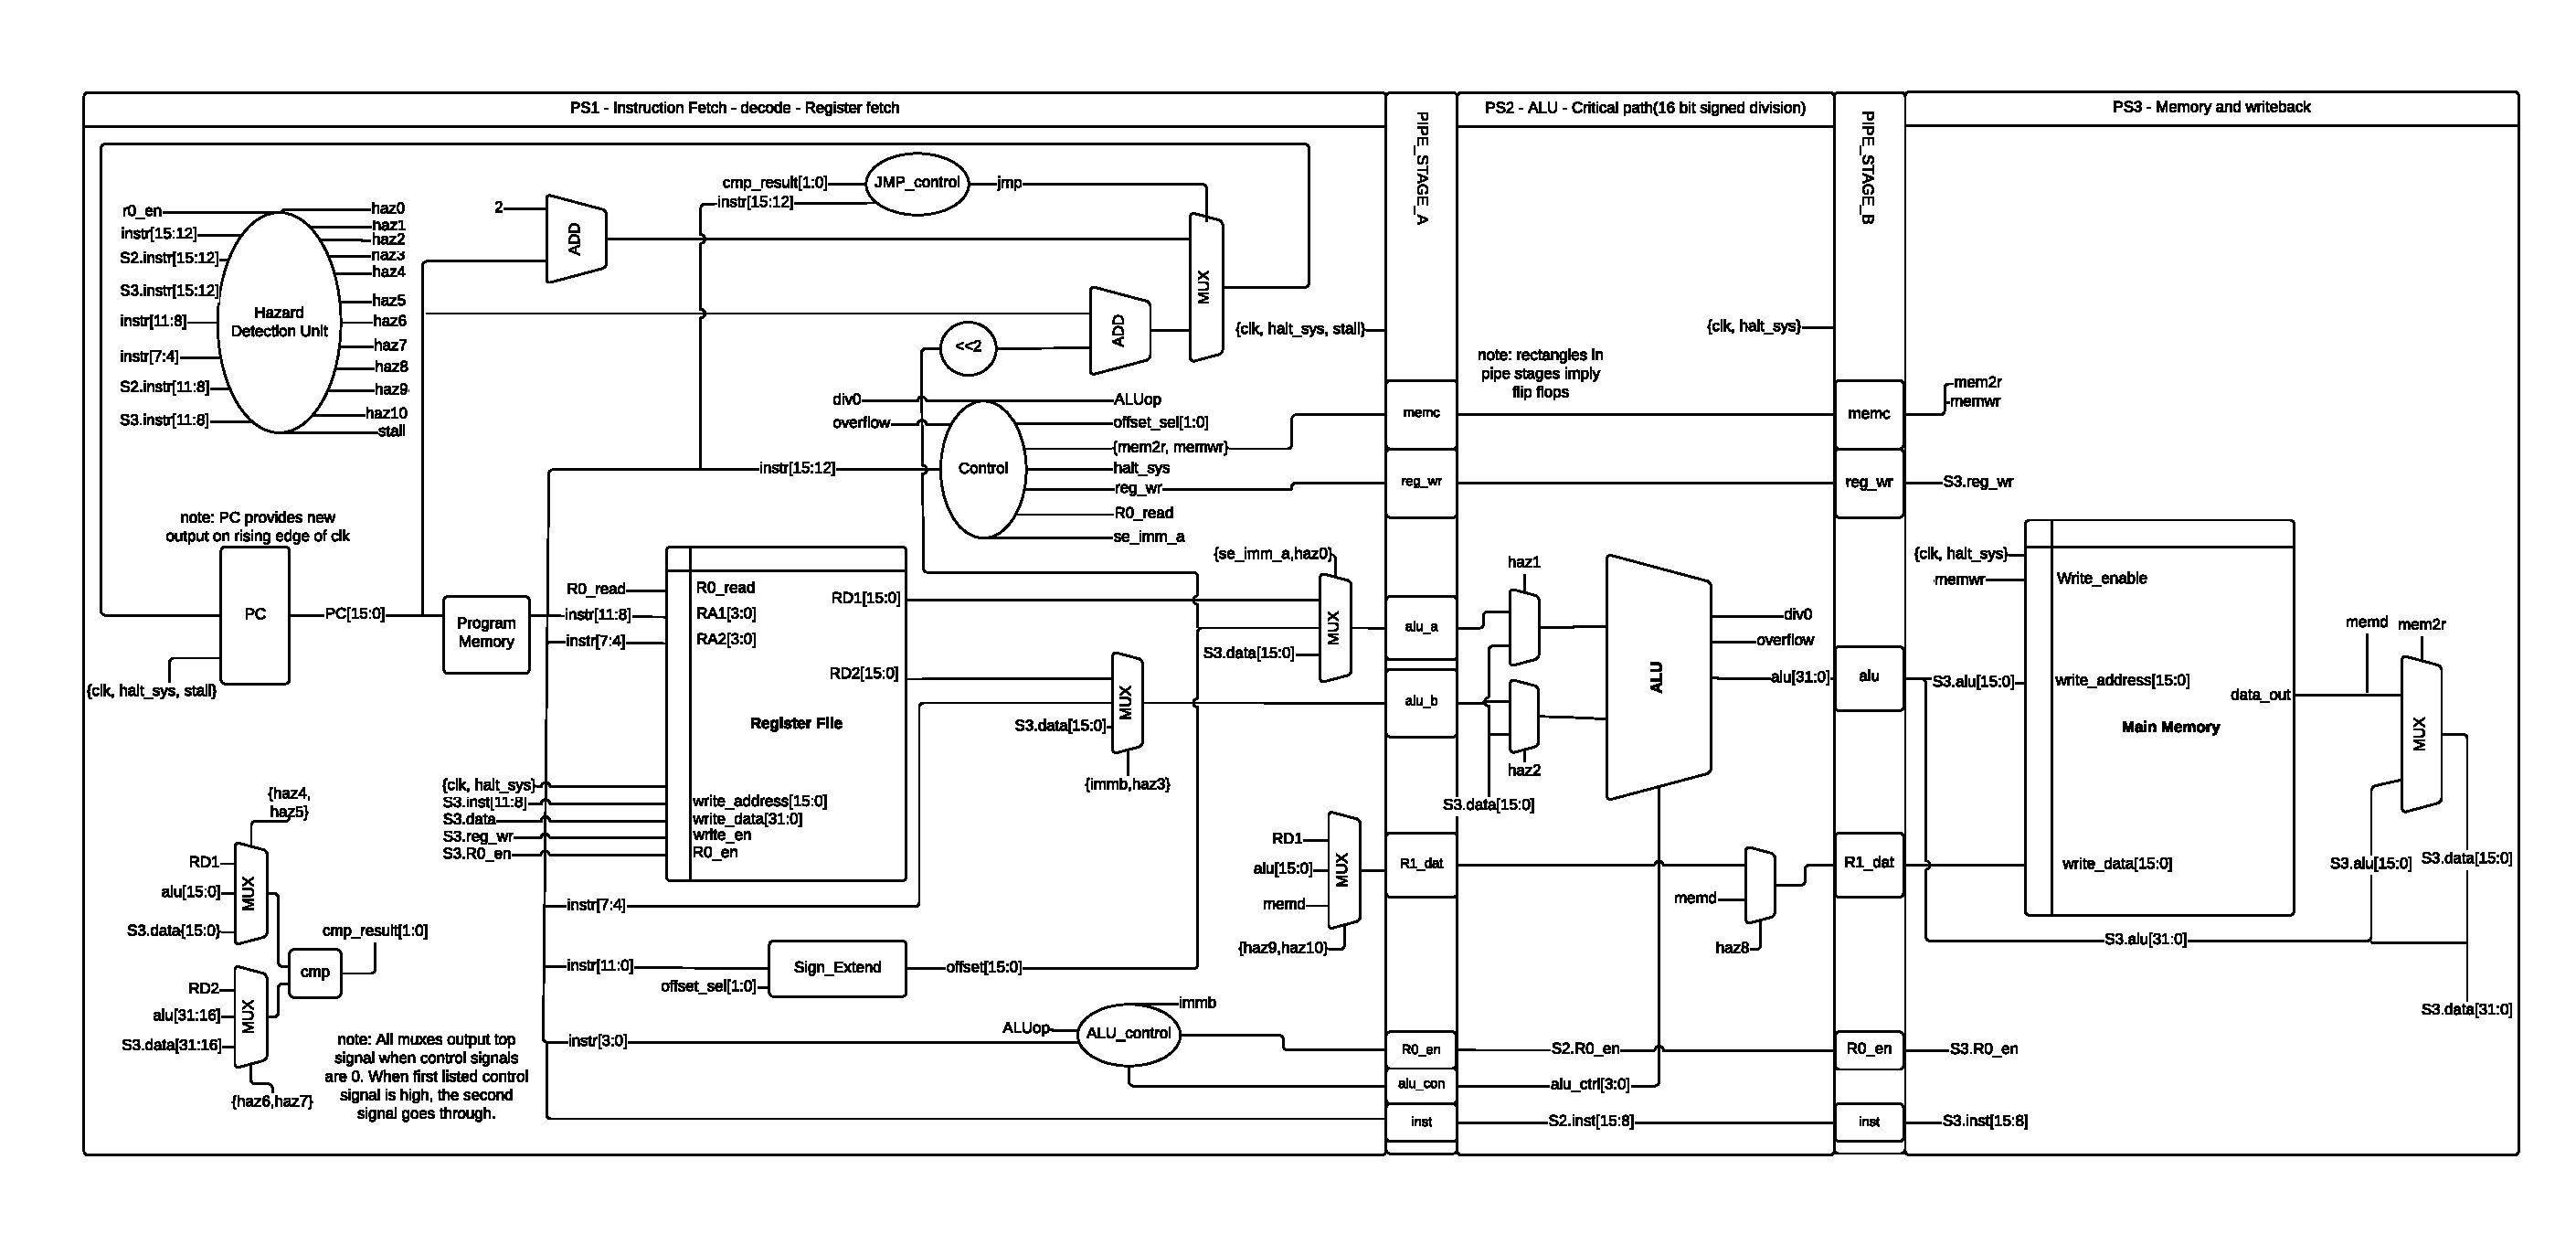
\includegraphics[angle=90,width=.63\textwidth]{./figures/142.pdf}
        \caption{Full CPU Pipeline Diagram}
        \label{fullschematic}
    \end{figure*}
    \FloatBarrier
	\onecolumn

    \section{Design Source Code}
        \subsection{Top Level}
        \lstinputlisting{../source/Design/top.sv}
        \lstinputlisting{../source/Design/types_pkg.sv}
        \lstinputlisting{../source/Design/alu_pkg.sv}

        \subsection{Stage One}
        \lstinputlisting{../source/Design/stage_one.sv}
        \lstinputlisting{../source/Design/adder.sv}
        \lstinputlisting{../source/Design/control_hazard_unit.sv}
        \lstinputlisting{../source/Design/control_jump.sv}
        \lstinputlisting{../source/Design/control_main.sv}      
        \lstinputlisting{../source/Design/comparator.sv}
        \lstinputlisting{../source/Design/control_alu.sv}
        \lstinputlisting{../source/Design/mem_program.sv}
        \lstinputlisting{../source/Design/mem_register.sv}
        \lstinputlisting{../source/Design/mux.sv}
        \lstinputlisting{../source/Design/reg_program_counter.sv}
        \lstinputlisting{../source/Design/shift_one.sv}
        \lstinputlisting{../source/Design/sign_extender.sv}      
        

        \subsection{Stage Two}
        \lstinputlisting{../source/Design/stage_two.sv}        
        \lstinputlisting{../source/Design/alu.sv}           
        
        \subsection{Stage Three}
        \lstinputlisting{../source/Design/stage_three.sv}
        \lstinputlisting{../source/Design/mem_main.sv}

    \section{Verification Source Code}
        \lstinputlisting{../source/Verif/alu_tb.sv}
        \lstinputlisting{../source/Verif/register_tb.sv}
        \lstinputlisting{../source/Verif/system_tb.sv}
        \lstinputlisting{../source/Verif/mux_tb.sv}
    
    \section{Build Scripts and utilities}
        \lstinputlisting[language = bash, label = imuangle]{../runsim.sh}
        \lstinputlisting[]{../vlogan_args.list}
        \lstinputlisting[]{../VCS_args.list}
\end{document}
